\documentclass[a4paper,12pt]{article}

\usepackage{../usfdvl}


\title{Worksheet 13}
\SetDocumentFooter{}{}


\begin{document}

\maketitle

\worksheetGroundRules

\worksheetSubmission

\assignmentInstructions

For the points below, first draw the Voronoi diagram (using any method, no need to show the steps). Next, use the Voronoi diagram to determine the Delaunay Triangulation. Show the algorithm using the following pages. Be sure to show all of the steps of your process.

\begin{itemize}
\item Determine the best/average/worst case big-O for the Delaunay Triangulation computation.


\end{itemize}


\begin{center}
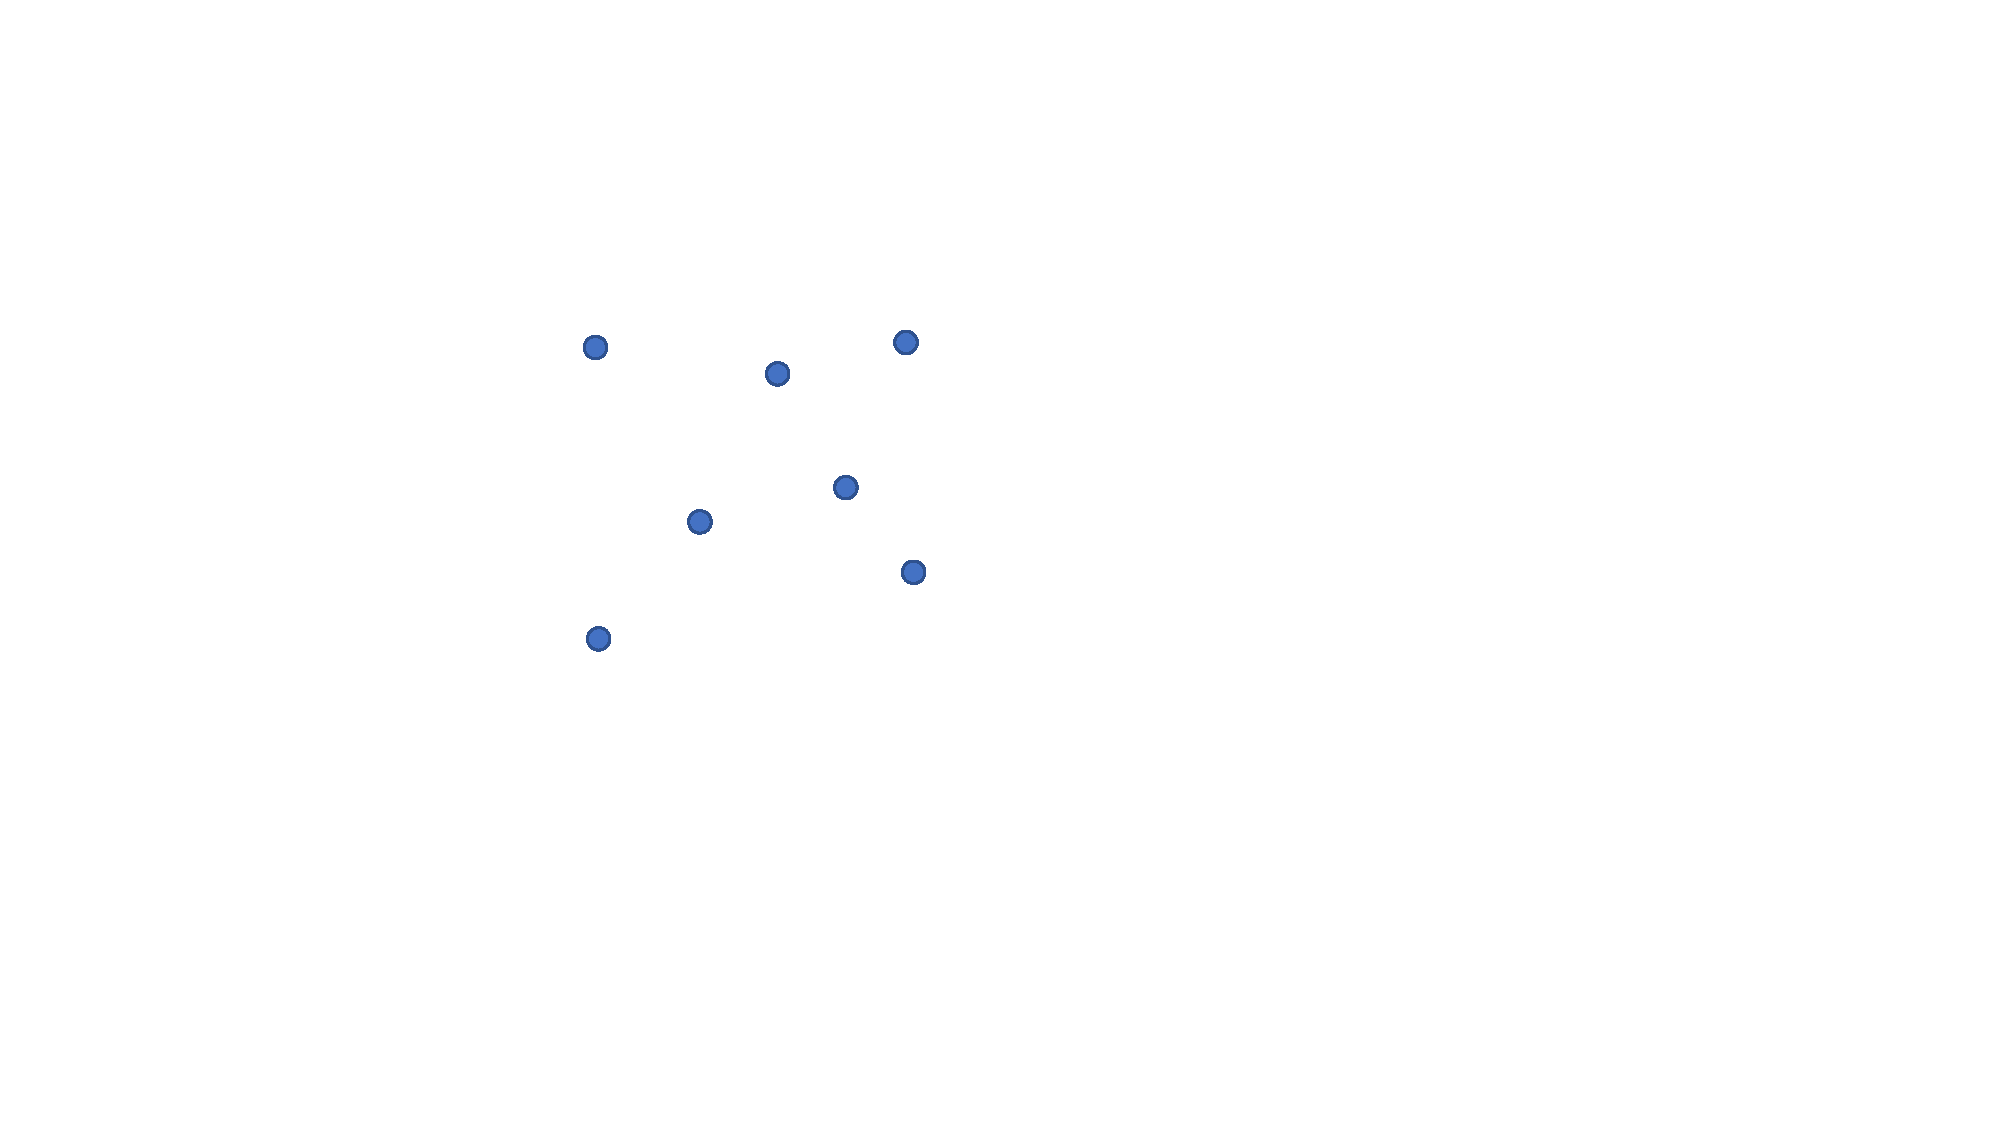
\includegraphics[width=0.65\linewidth]{../images/voronoi7.pdf}
\end{center}



\newpage

\begin{tabular}{|c|c|}
\hline
\hspace{10pt}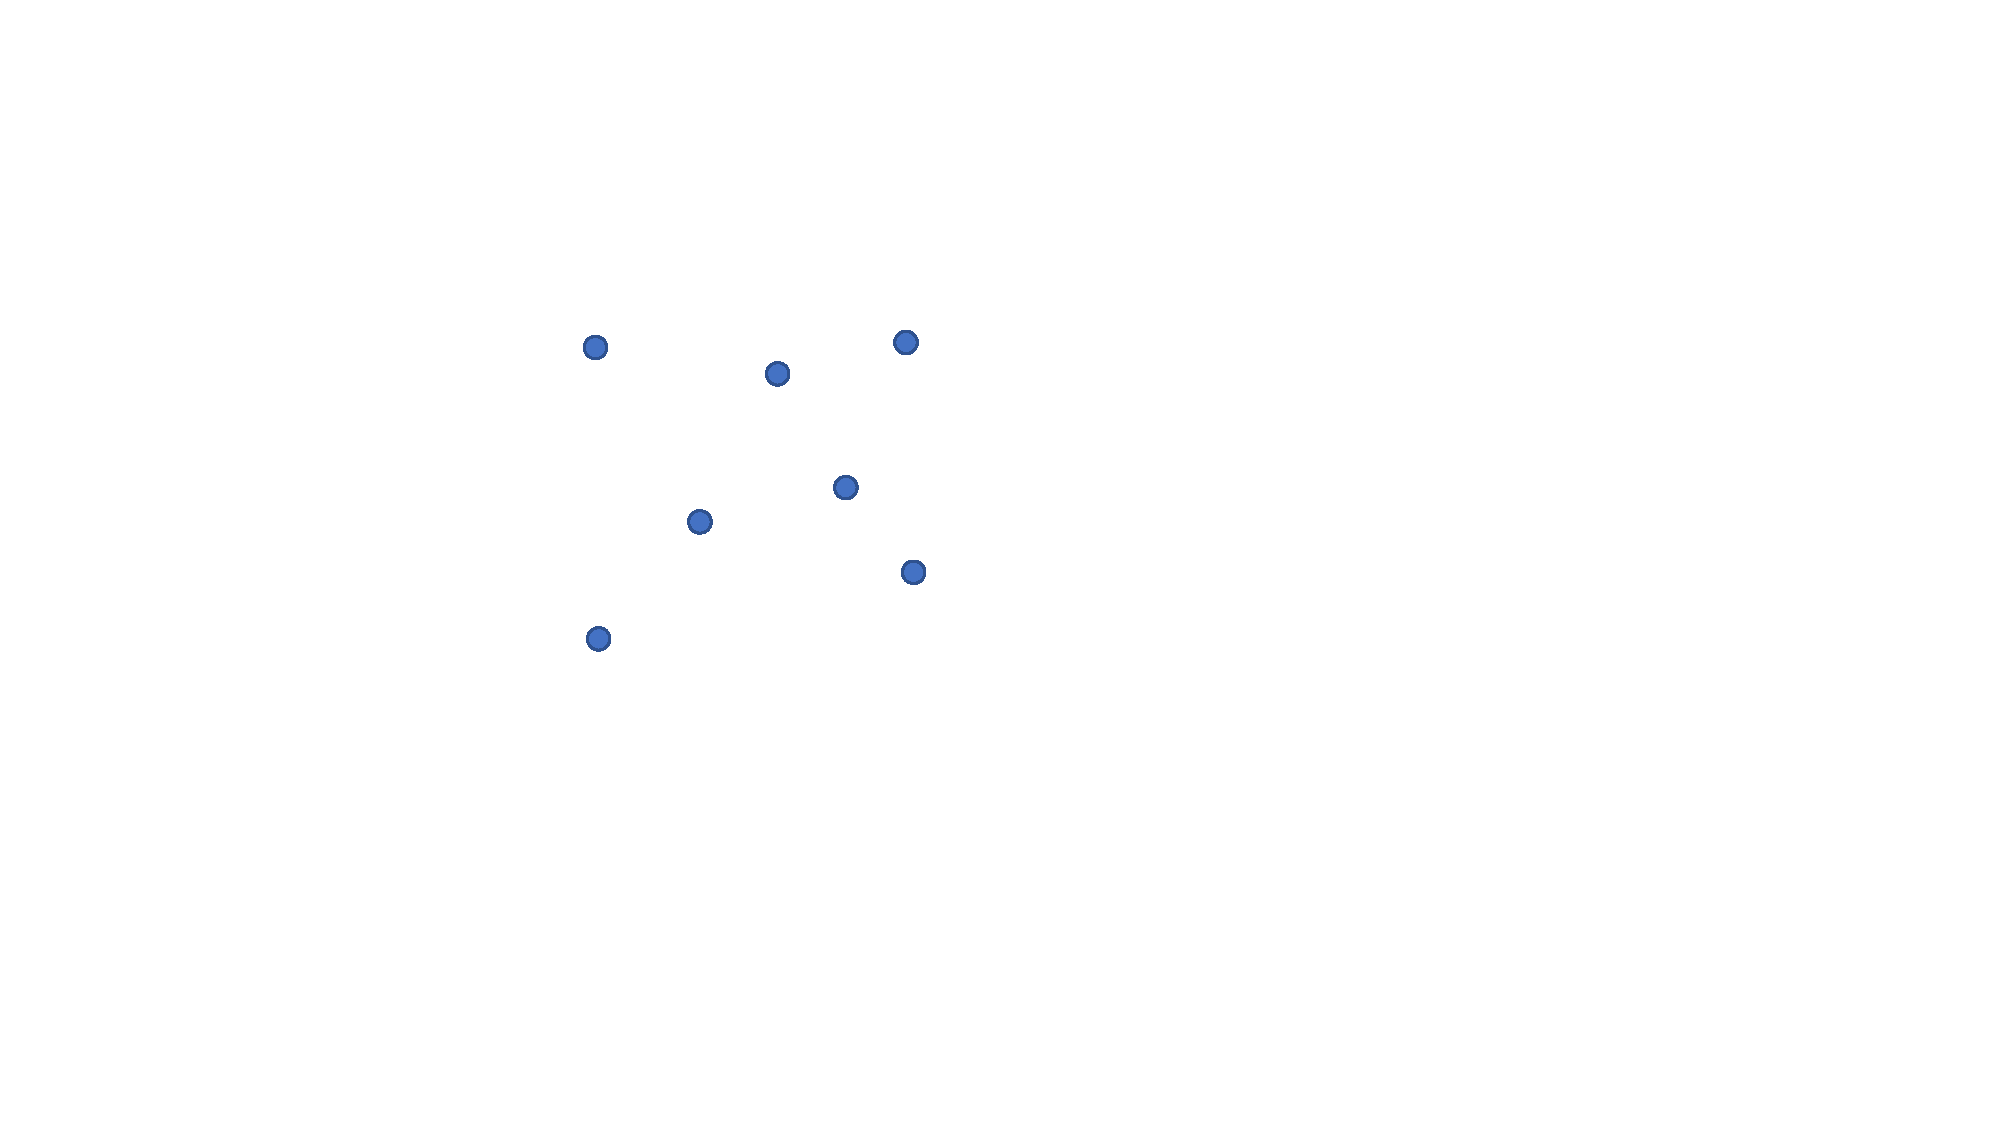
\includegraphics[width=0.425\linewidth]{../images/voronoi7.pdf}\hspace{10pt} & \hspace{10pt}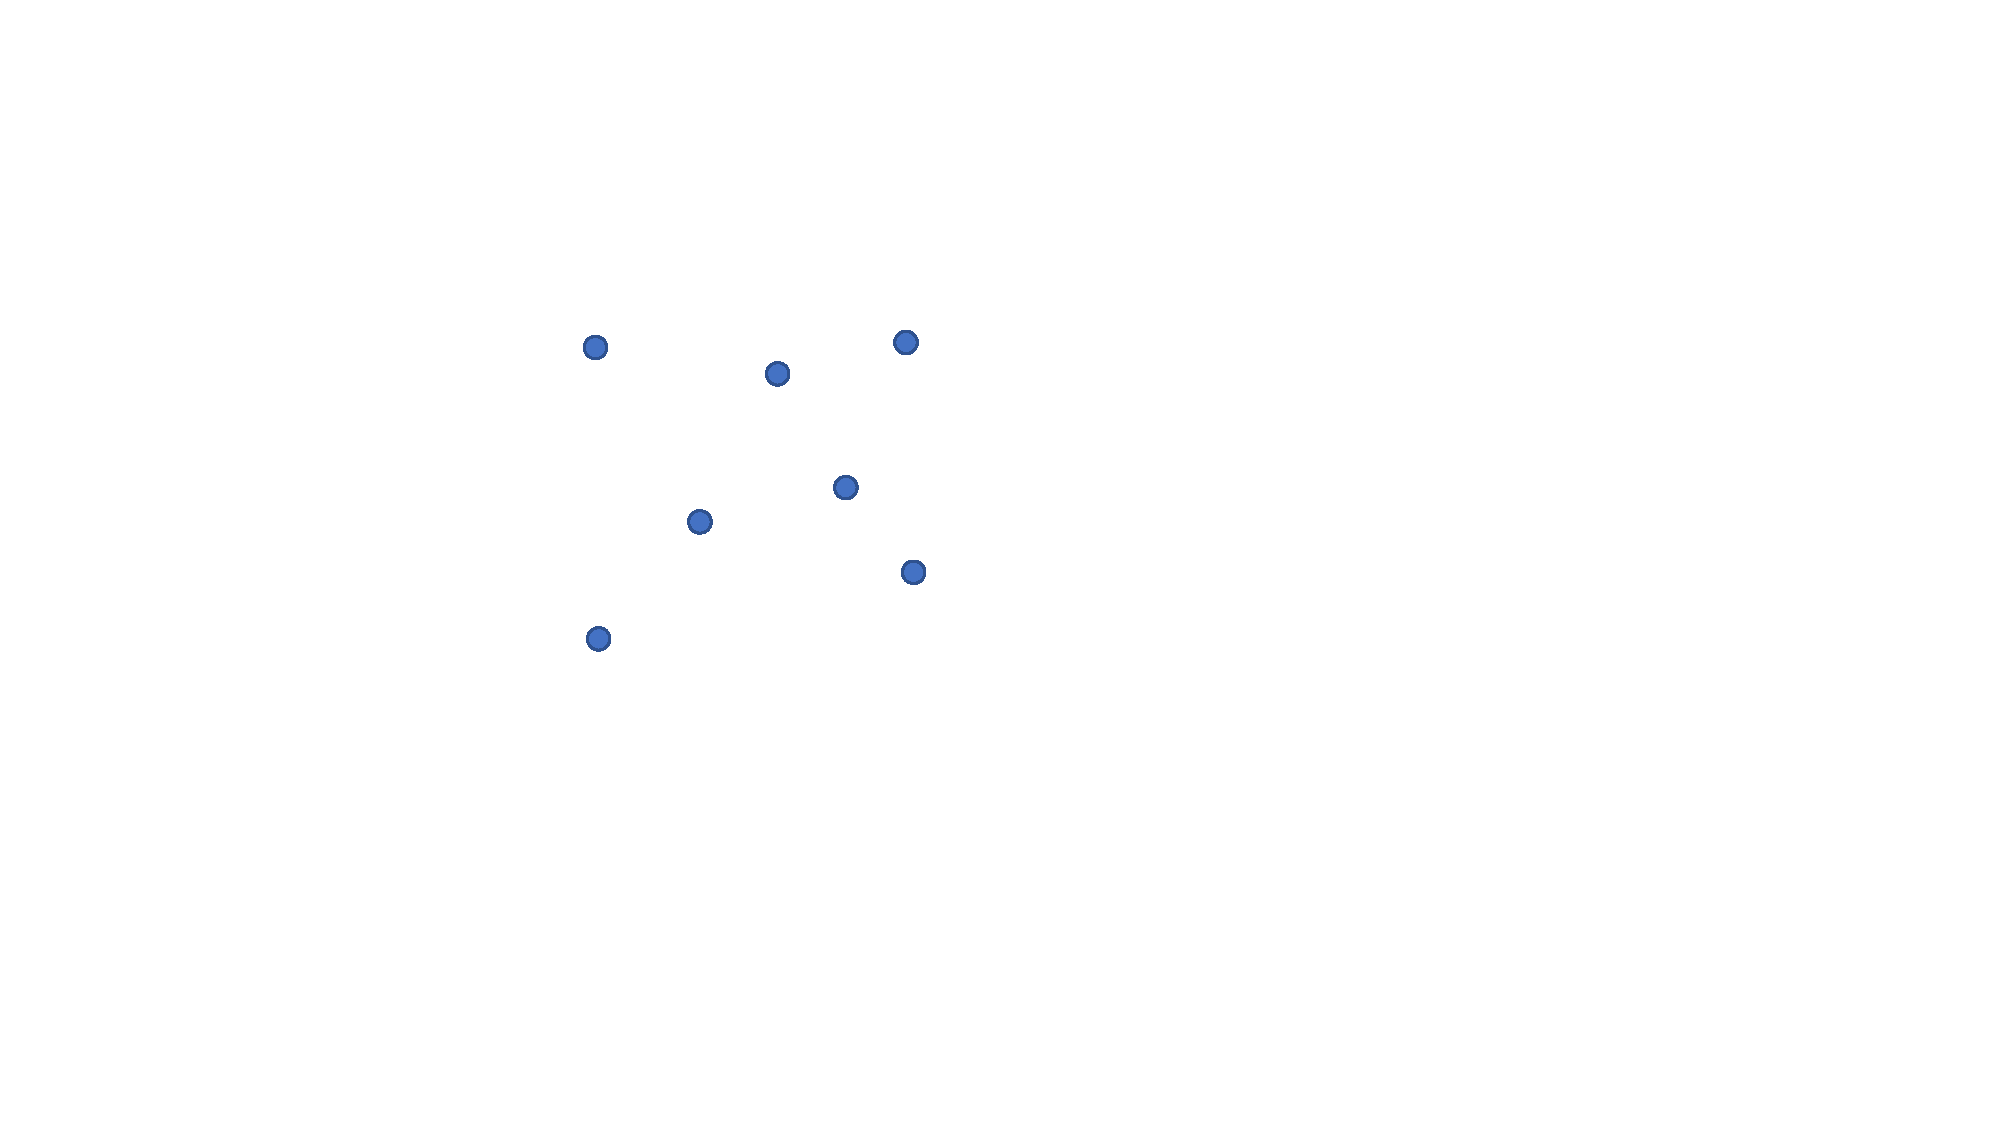
\includegraphics[width=0.425\linewidth]{../images/voronoi7.pdf}\hspace{10pt} \\
Voronoi Diagram & Delaunay Triangulation \\
\hline
\hspace{10pt}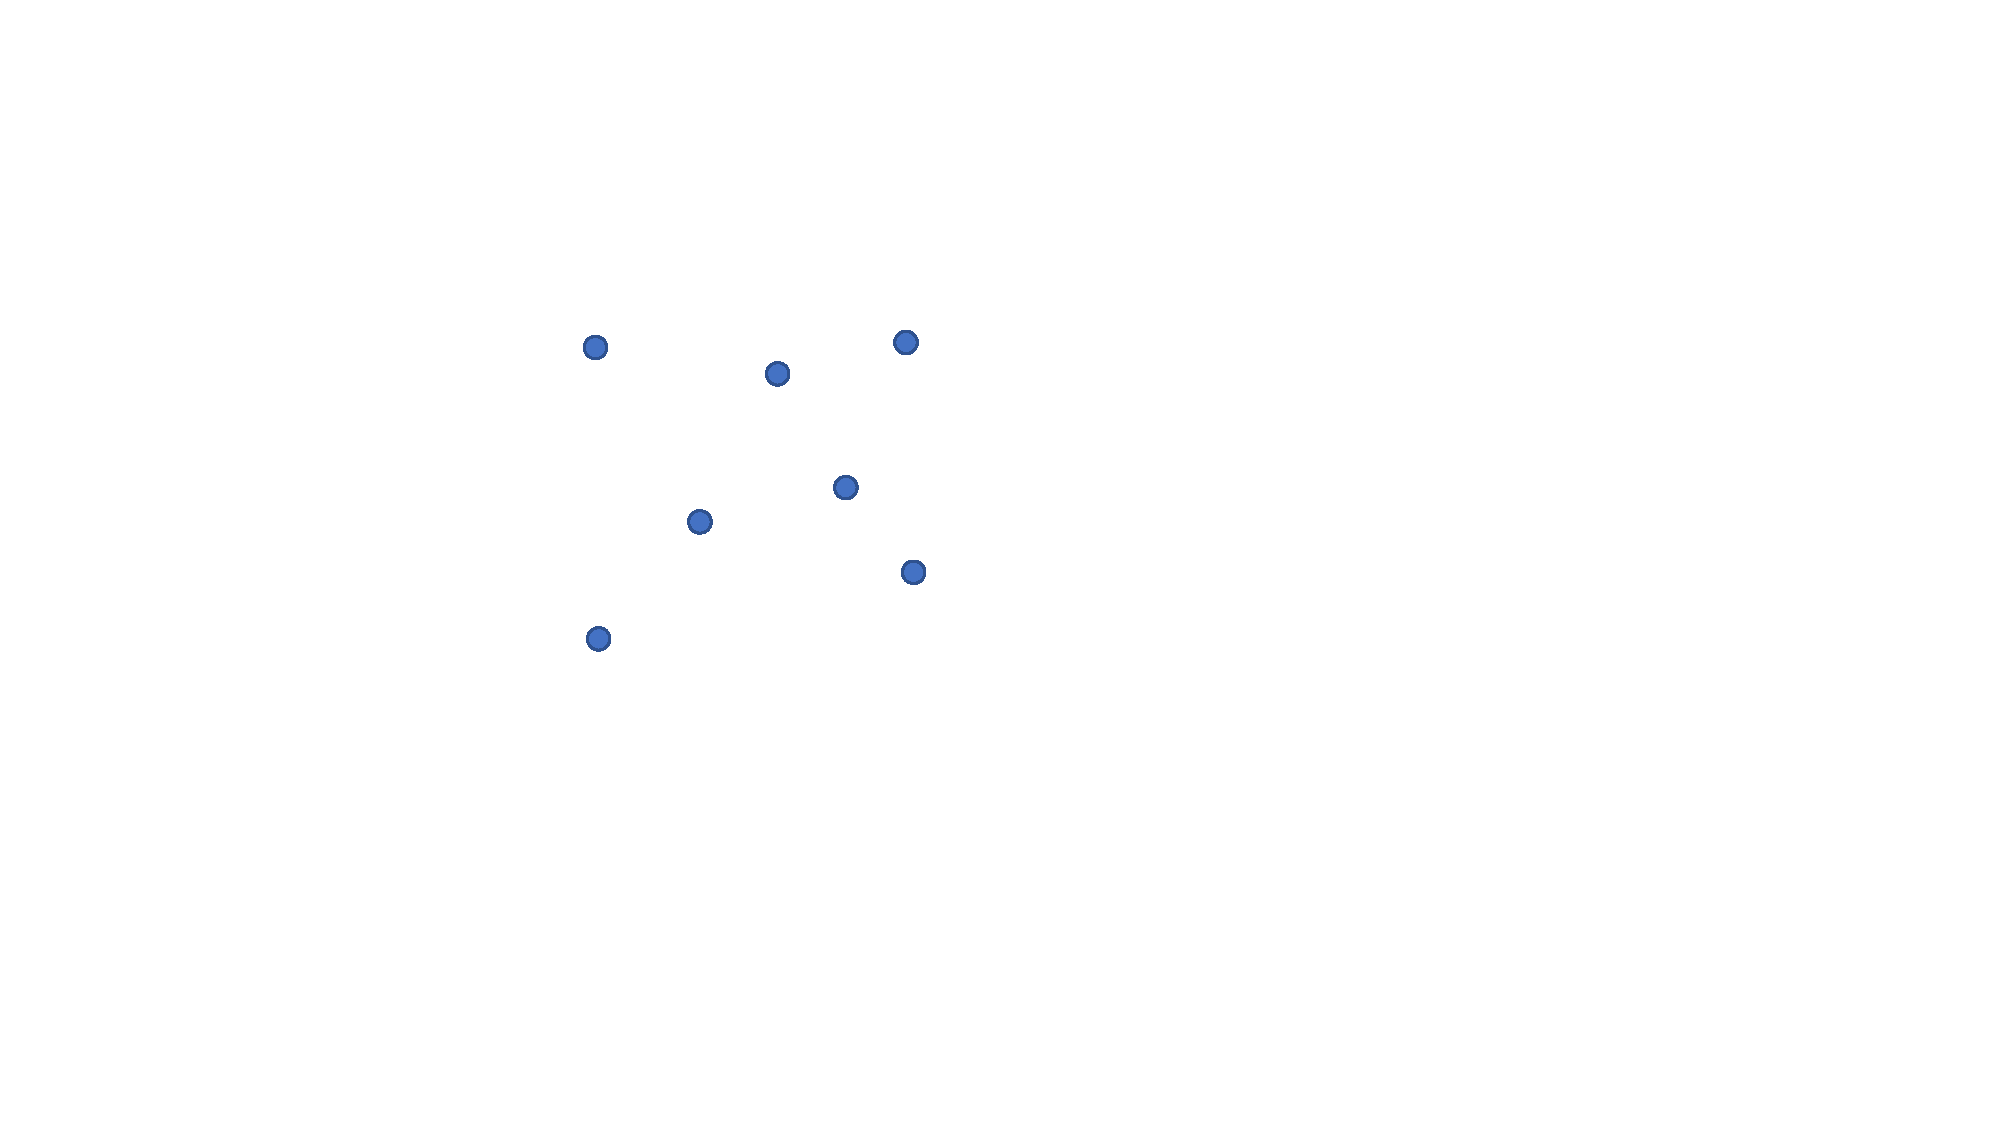
\includegraphics[width=0.425\linewidth]{../images/voronoi7.pdf}\hspace{10pt} & \hspace{10pt}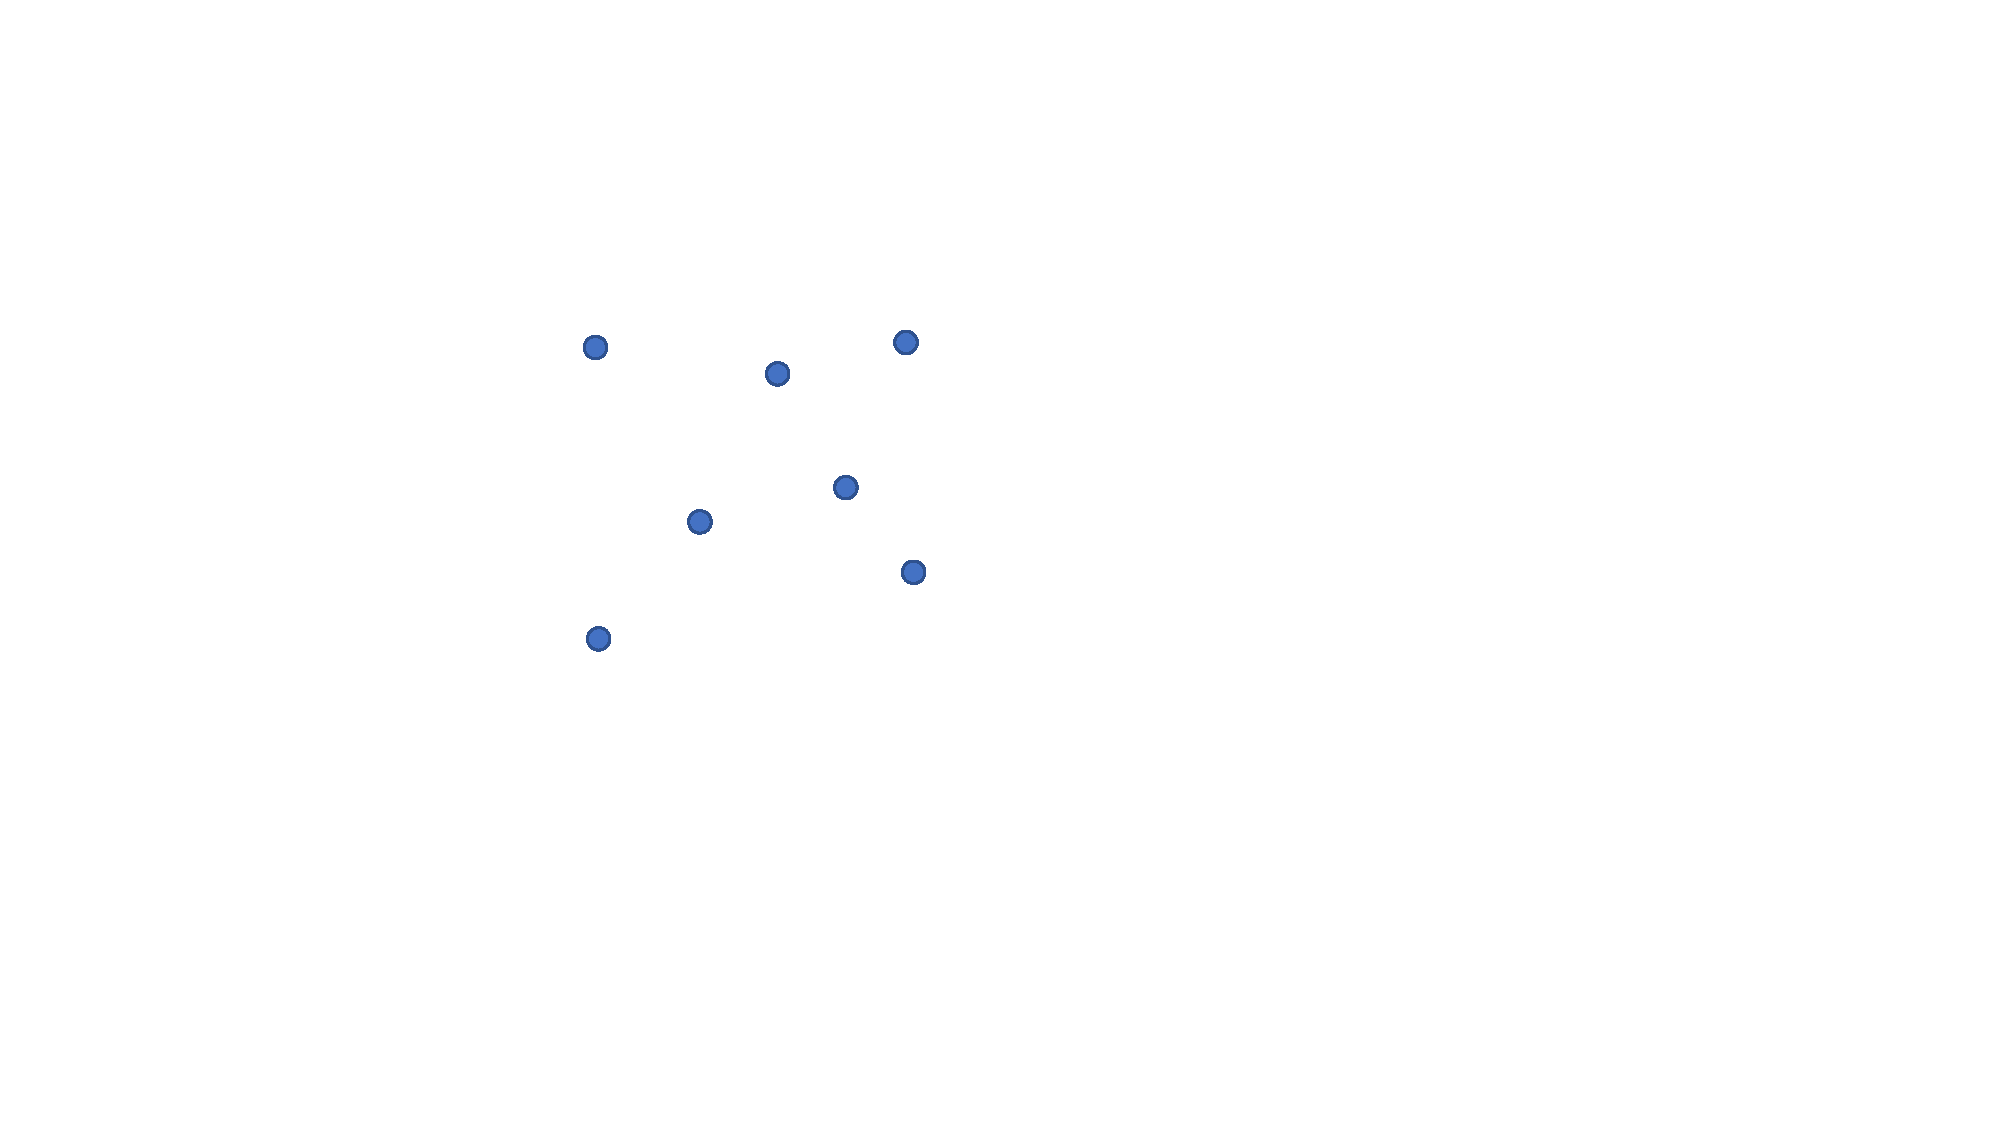
\includegraphics[width=0.425\linewidth]{../images/voronoi7.pdf}\hspace{10pt} \\
Delaunay Triangulation & Delaunay Triangulation \\
\hline
\end{tabular}

\begin{tabular}{|c|c|}
\hline
\hspace{10pt}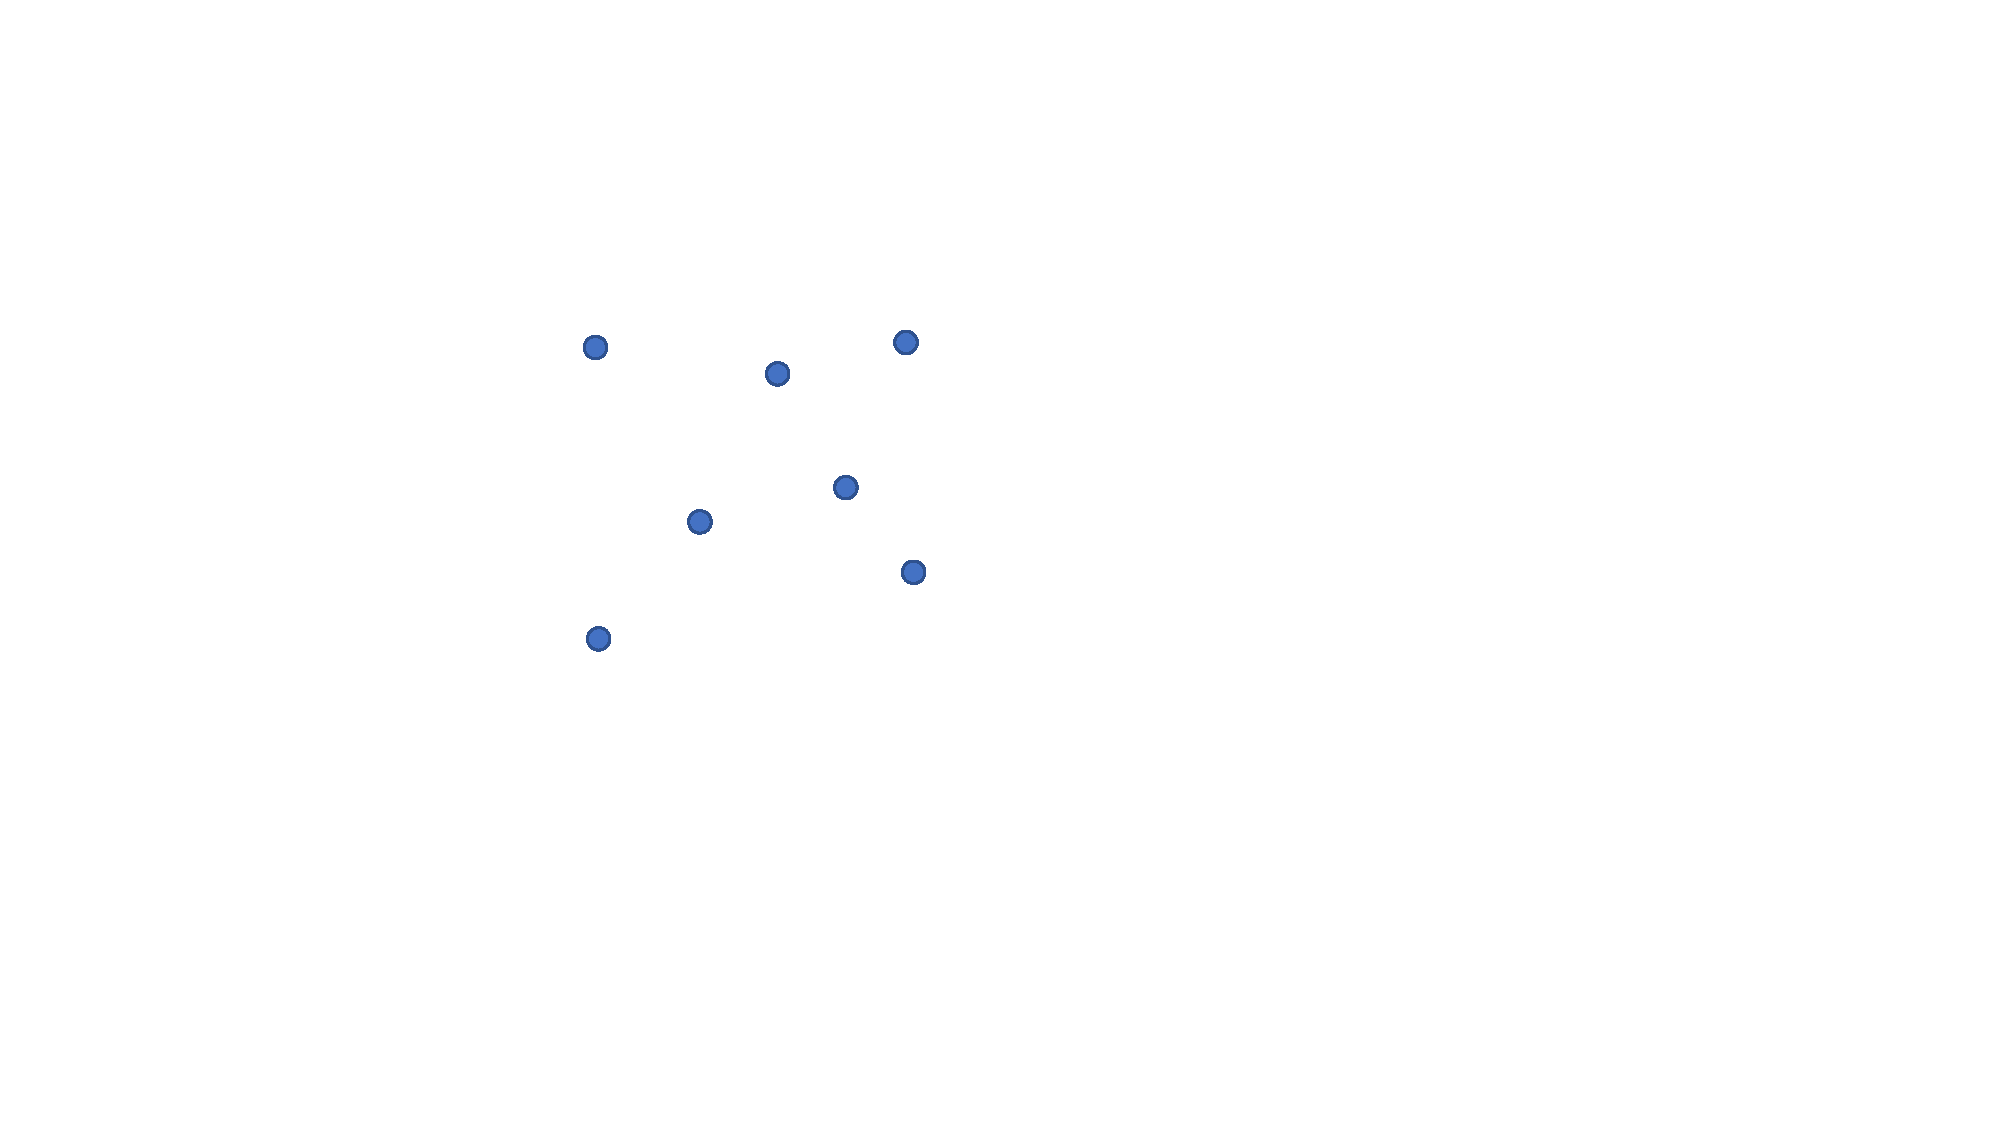
\includegraphics[width=0.425\linewidth]{../images/voronoi7.pdf}\hspace{10pt} & \hspace{10pt}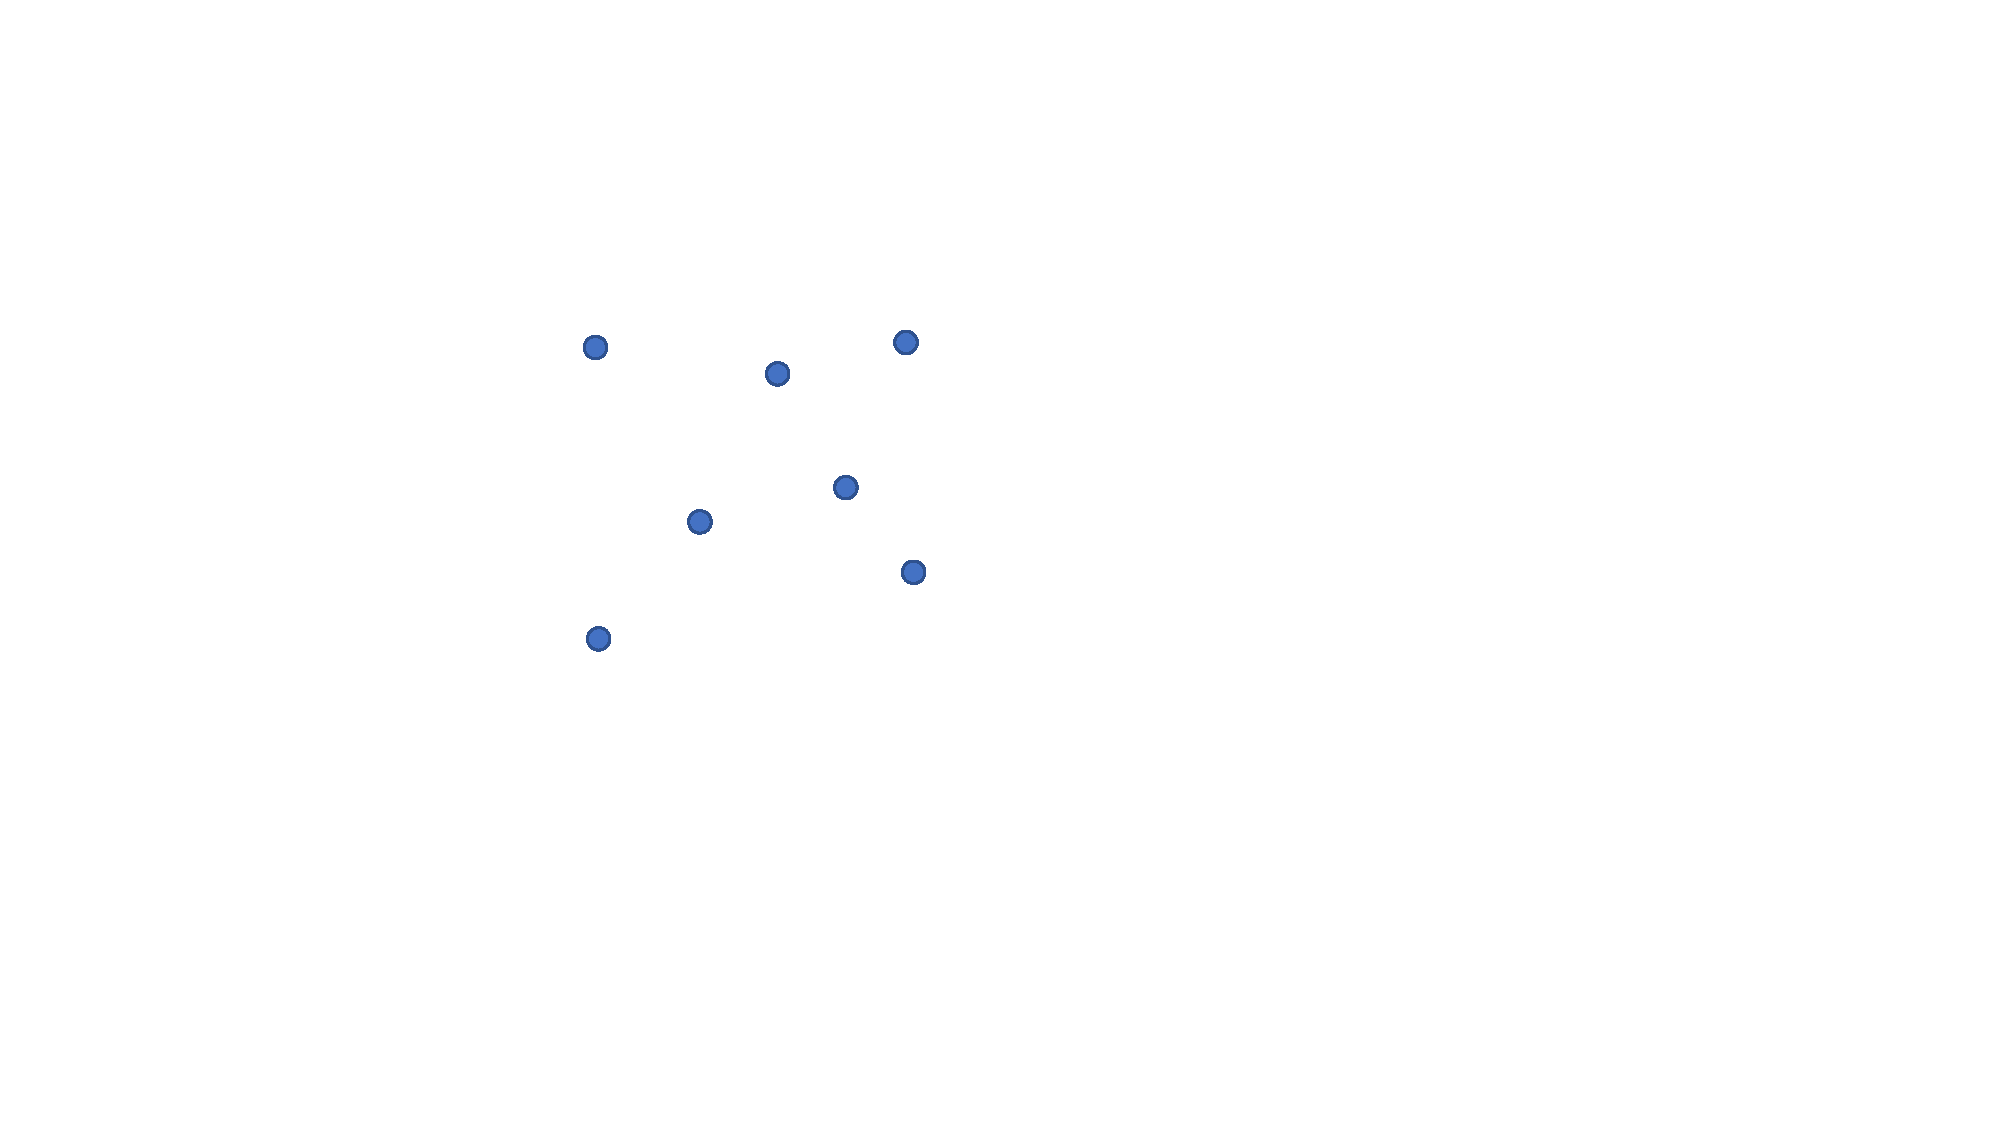
\includegraphics[width=0.425\linewidth]{../images/voronoi7.pdf}\hspace{10pt} \\
Delaunay Triangulation & Delaunay Triangulation \\
\hline
\hspace{10pt}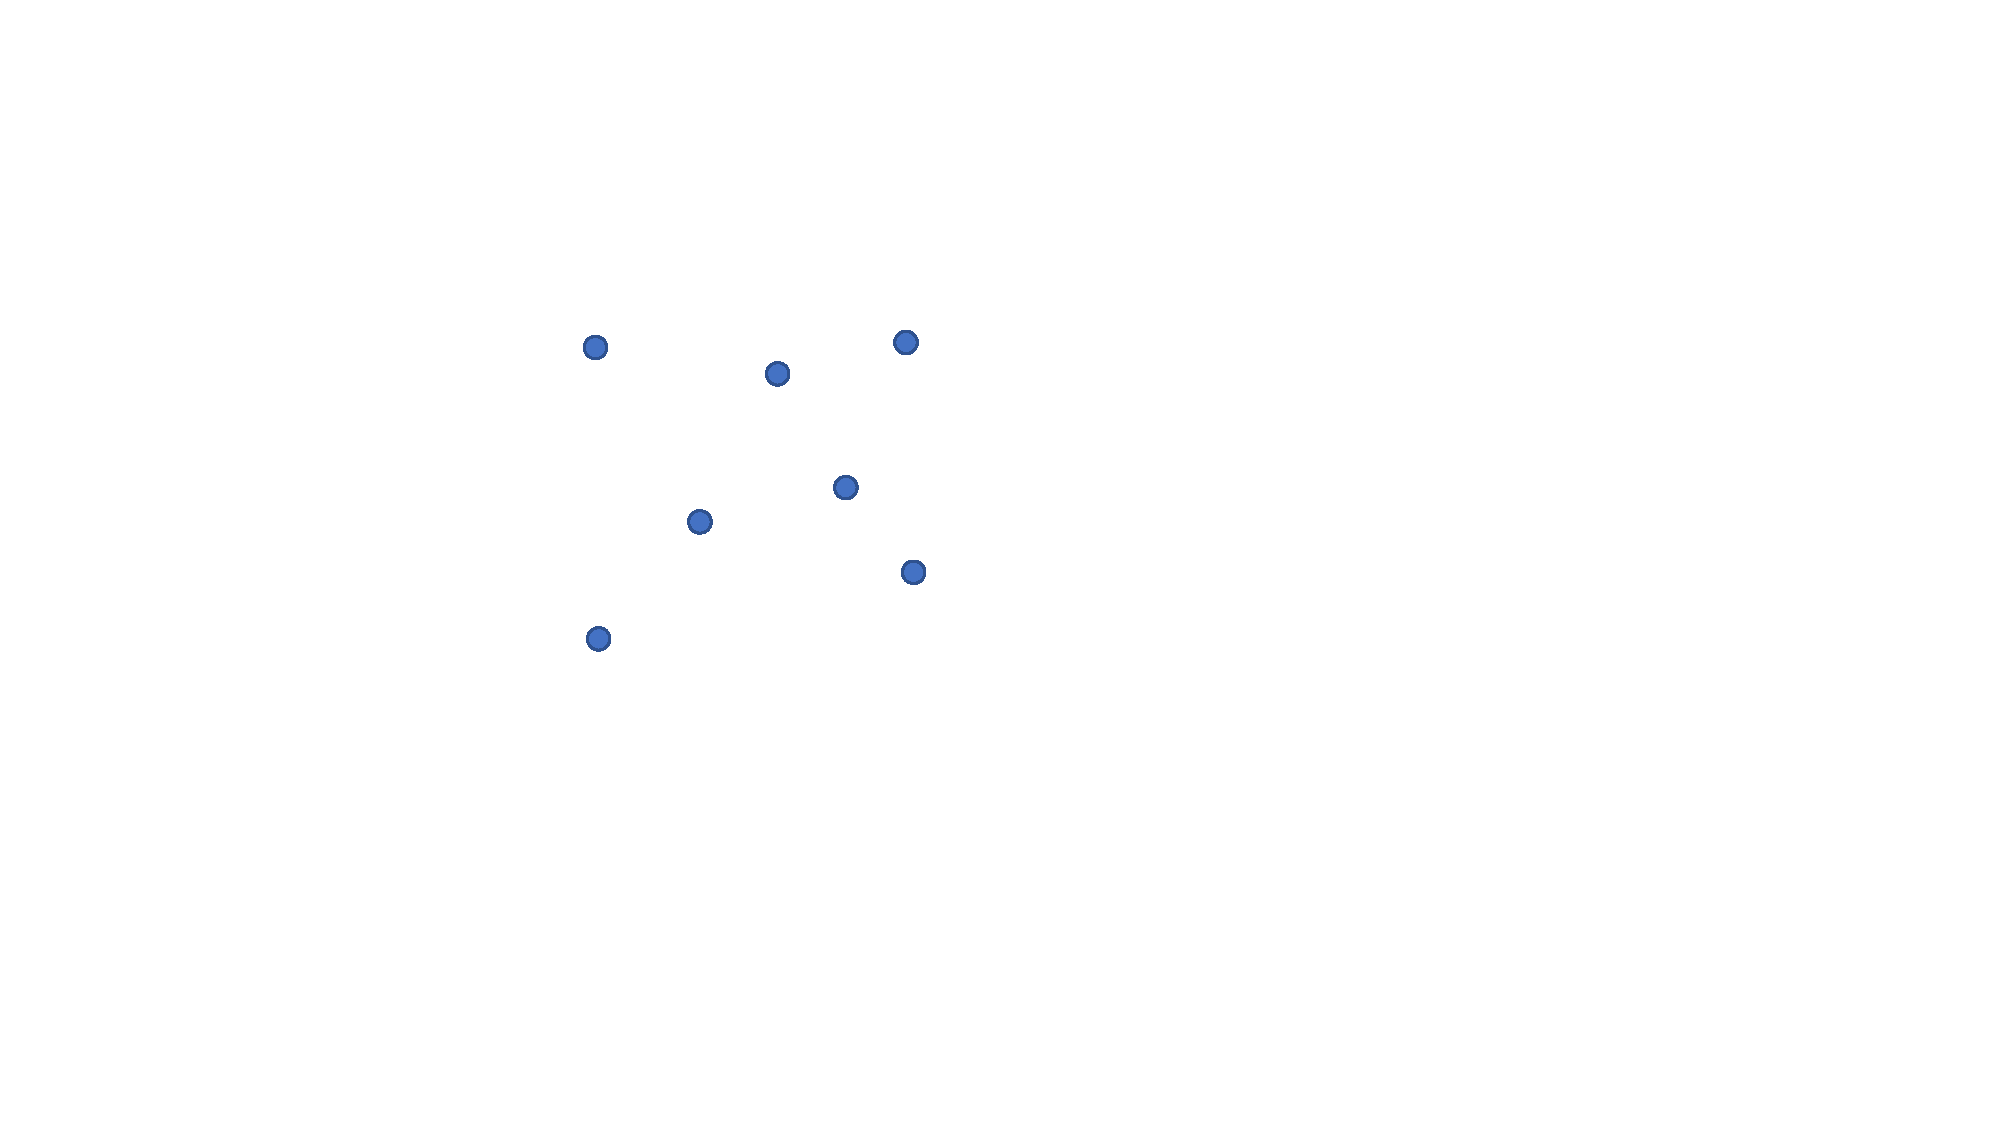
\includegraphics[width=0.425\linewidth]{../images/voronoi7.pdf}\hspace{10pt} & \hspace{10pt}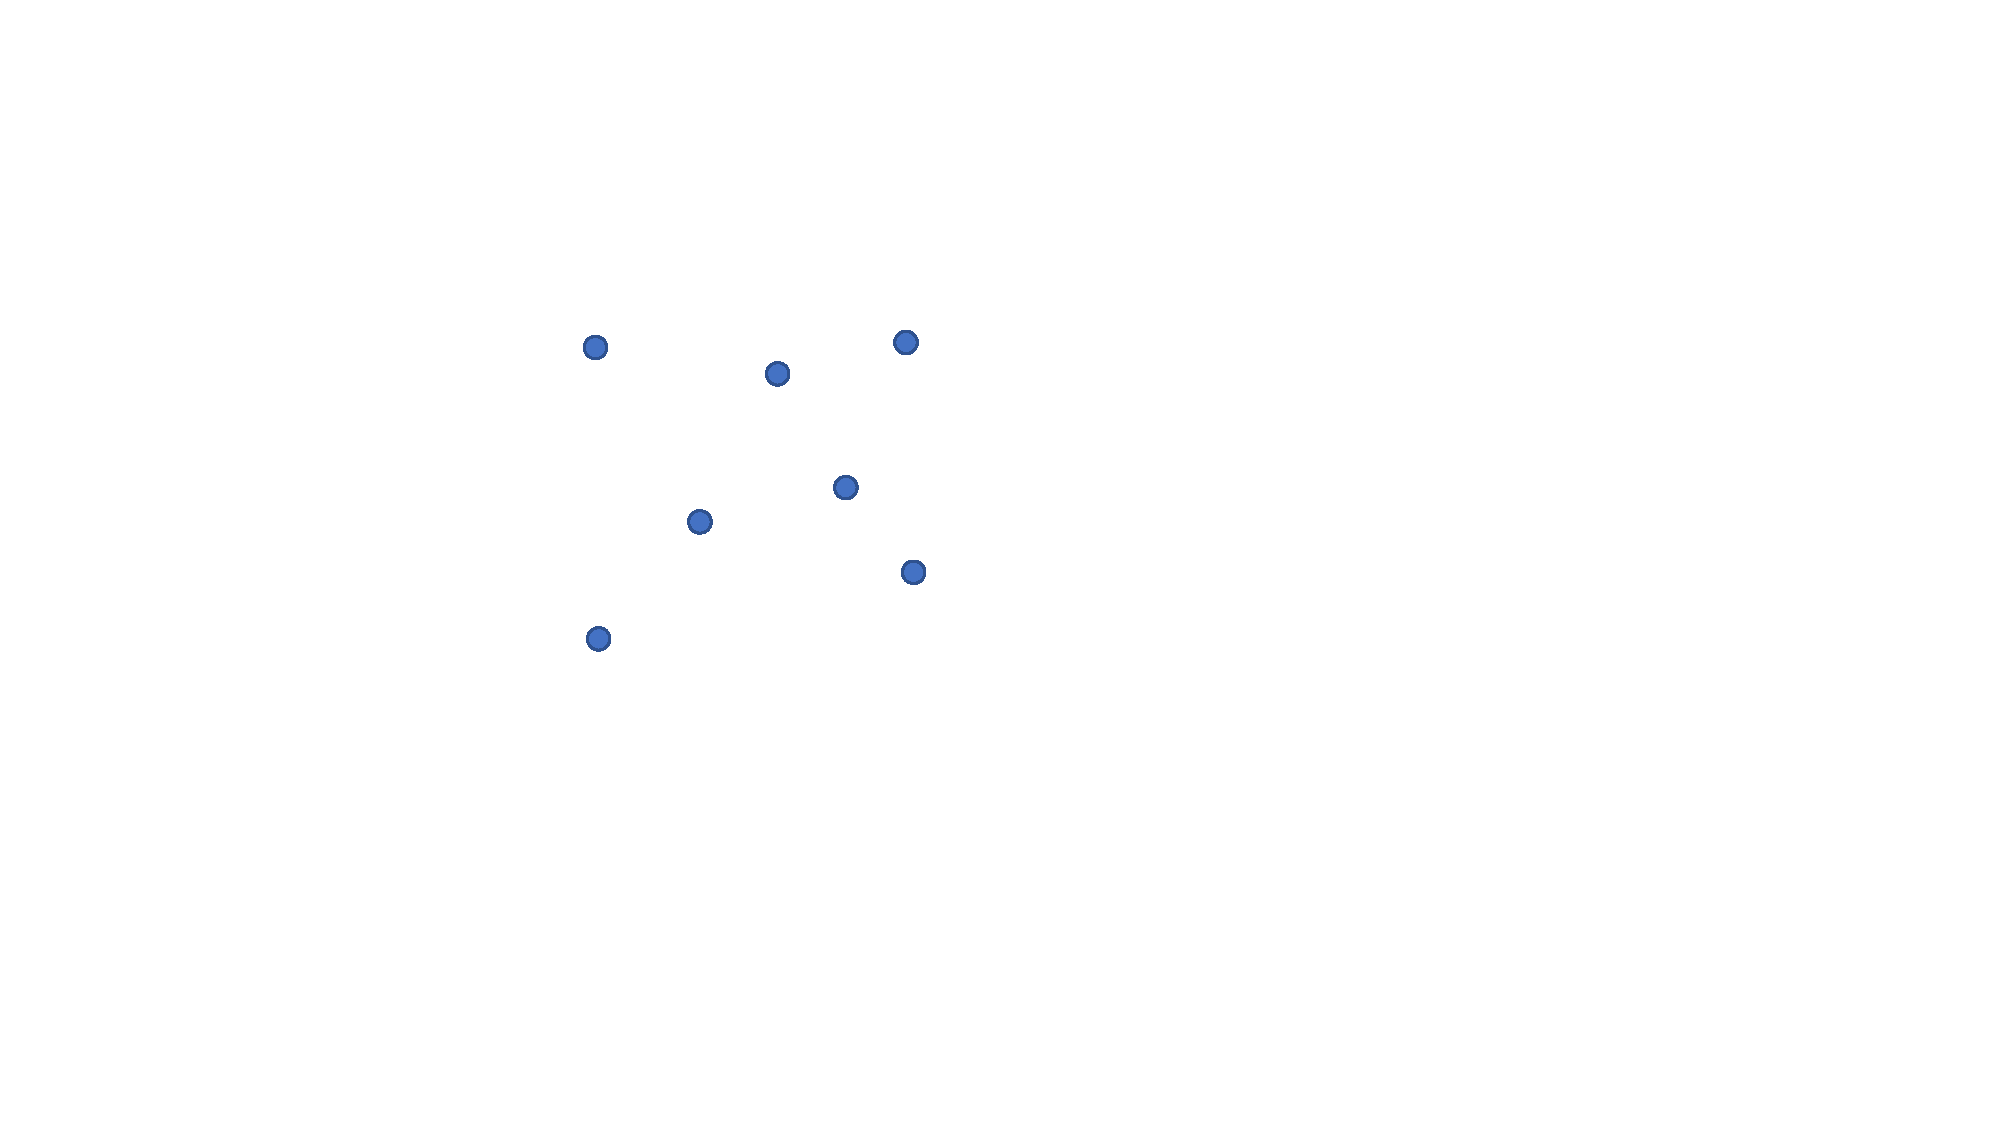
\includegraphics[width=0.425\linewidth]{../images/voronoi7.pdf}\hspace{10pt} \\
Delaunay Triangulation & Delaunay Triangulation \\
\hline
\end{tabular}





\end{document}



